\subsection{PCB}
\label{sec:PCB}

Im nachfolgenden Kapitel wird näher erläutert wie das PCB aufgebaut ist und worauf geachtet wurde.

Grundsätzlich ist das Board in zwei fundamentale Teile eingeteilt (ersichtlich in Abbildung \ref{fig:PCB_GNDVDD}).  Den Digital-Teil inklusive Speisung, Microcontroller und den digitalen Schnittstellen. Und den Analog-Teil mit dem Codec und den verschiedenen Ein- und Ausgängen. In beiden Teilen wird rückseitig separat die Ground-Fläche geführt. Die beiden Flächen sind, wie in \ref{par:GND} erläutert, an genau einem Punkt durch einen $0\Omega$ Widerstand verbunden. Um die Speisungen grösstmöglich zu führen sind vorderseitig die beiden Teile mit 3.3VA beziehungsweise 3.3VD ausgegossen (nachdem alle Verbindungen gezogen worden sind).

\begin{figure} [H]
\begin{center}
 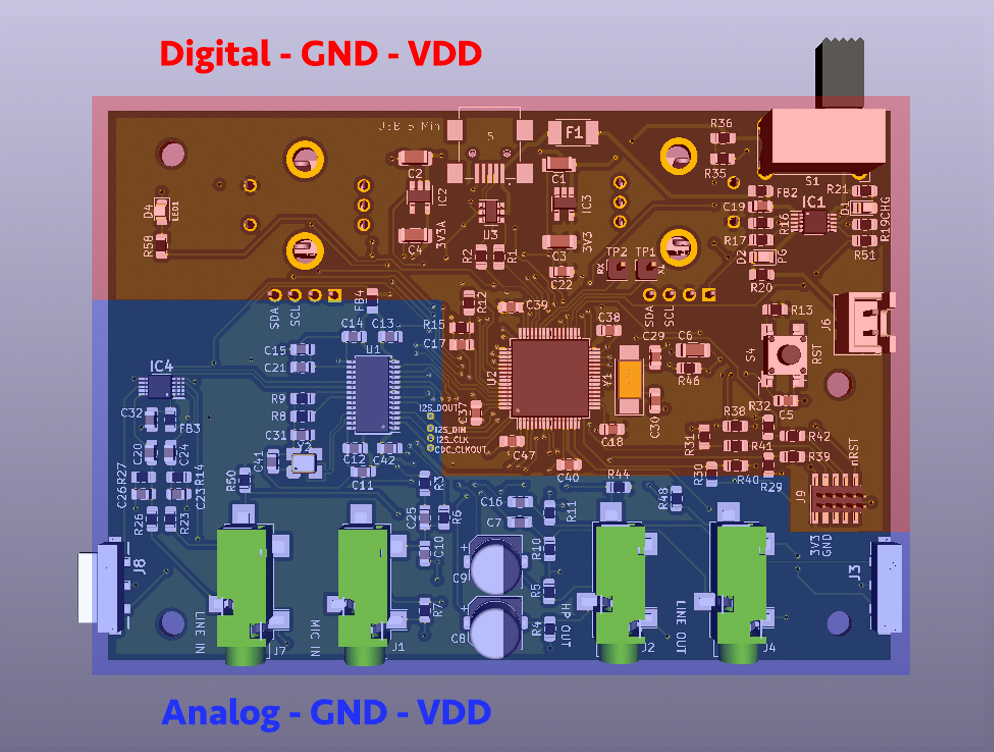
\includegraphics[scale=0.37]{../graphics/PCB-Layout_GNDVDD.jpg}
 \caption{Die Unterteilung des PCBs in Analog- und Digital-Teil}
\label{fig:PCB_GNDVDD}
\end{center}
\end{figure}

Im Speisungs-Teil ist wichtig, dass keine Speisungs-Schleifen entstehen. Die  Speiseleitungen sind zudem doppelt so breit wie die restlichen Leitungen (0.5mm), um den maximalen Strom von 500mA auszuhalten.

\begin{figure} [H]
\begin{center}
 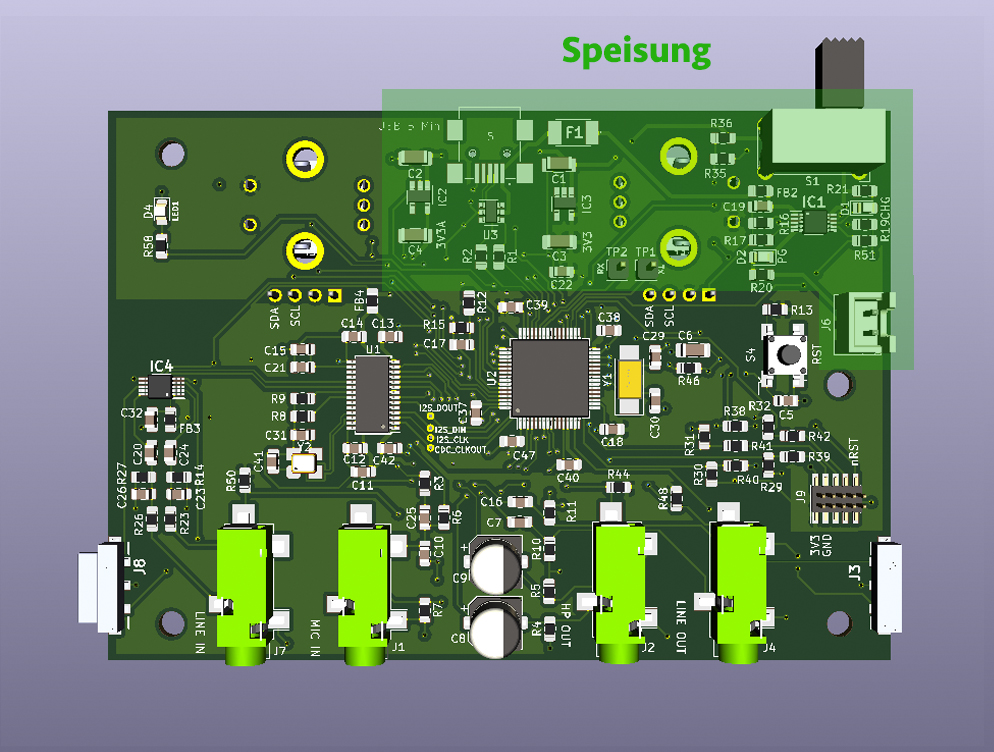
\includegraphics[scale=0.37]{../graphics/PCB-Layout_PWR.jpg}
 \caption{Die Speisung des PCBs mit der Mini-USB-Buchse, dem Lade-IC für den Akku sowie den beiden LDOs für Digital- sowie Analog-Teil}
\label{fig:PCB_PWR}
\end{center}
\end{figure}

Die räumliche Trennung verschiedener Teile auf dem PCB sollte mögliche gegenseitige Wechselwirkungen vermeiden oder zumindest vermindern. Speziell die Speisung und der Audio-Teil sind getrennt. Im Speisungs-Teil fliessen sicher die grössten Ströme auf dem ganzen Print, was mögliche EMV-Komplikationen nach sich ziehen kann. Im Audio-Teil würden im schlimmsten Fall solche Induktions-Spannungen als Signal interpretiert werden. Deswegen sind diese beiden Teile weitmöglichst voneinander, in den beiden Ecken, platziert.

\begin{figure} [H]
\begin{center}
 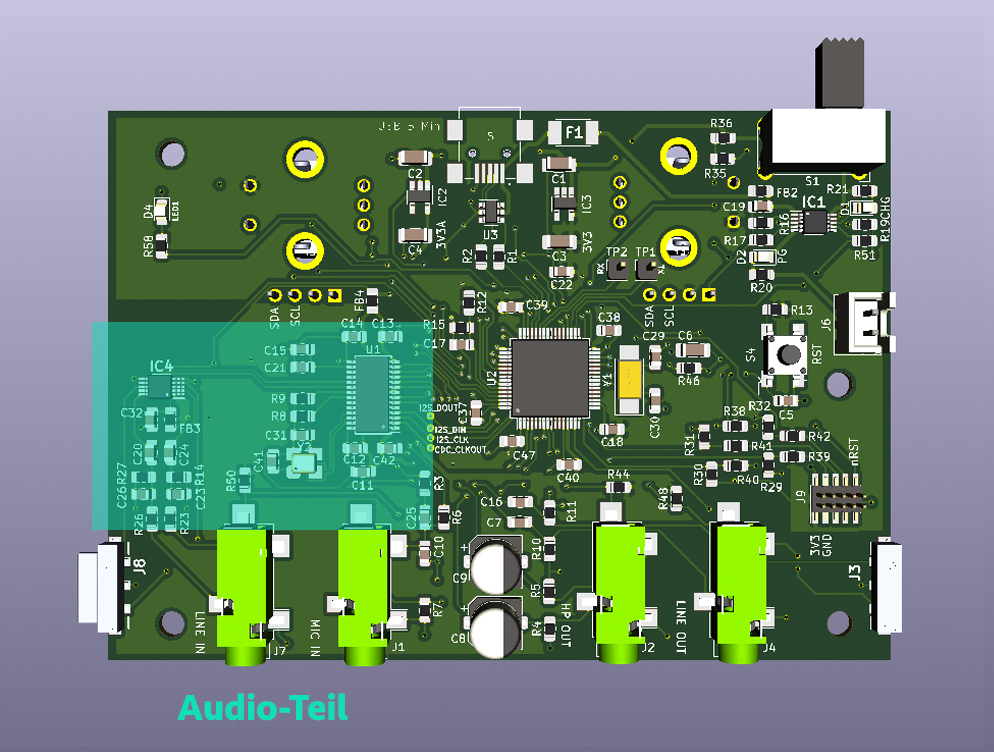
\includegraphics[scale=0.37]{../graphics/PCB-Layout_AUDIO.jpg}
 \caption{Der Audio-Teil mit dem Codec, dem Audio-Switch, dem 12.28MHz Quartz sowie der äusseren Beschaltung der Ein- und Ausgänge}
\label{fig:PCB_AUDIO}
\end{center}
\end{figure}

Im Audio-Teil sind zusätzliche Messpunkte zur Überprüfung der I\textsuperscript{2} S Kommunikation hinzugefügt, welche nur für den Prototyp vorgesehen sind. 

\begin{figure} [H]
\begin{center}
 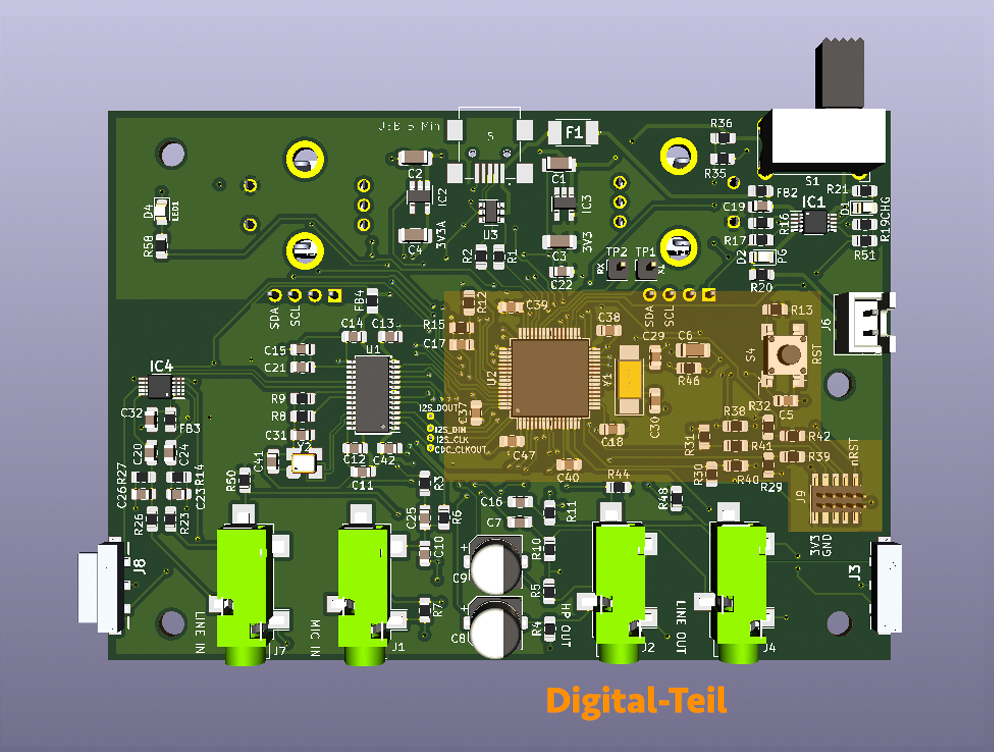
\includegraphics[scale=0.37]{../graphics/PCB-Layout_DGTL.jpg}
 \caption{Der Digital-Teil mit dem Mikrokontroller, dem 8MHz Quartz und der JTAG-Schnittstelle}
\label{fig:PCB_DGTL}
\end{center}
\end{figure}

Im Digital-Teil sind vor allem die Stützkondensatoren der Speisung und der 8MHz Quartz möglichst nahe an den Pins des Microcontrollers platziert. Für den Clock ist ein differenzielles Leitungspaar gezogent, ein Befehl in KiCad welcher bewirkt dass die beiden Leitungen exakt gleich lang werden. Dieser Befehl ist ebenfalls für den 12.28MHz des Audio-Teils und die Datenleitungen des USB-Steckers implementiert.

\begin{figure} [H]
\begin{center}
 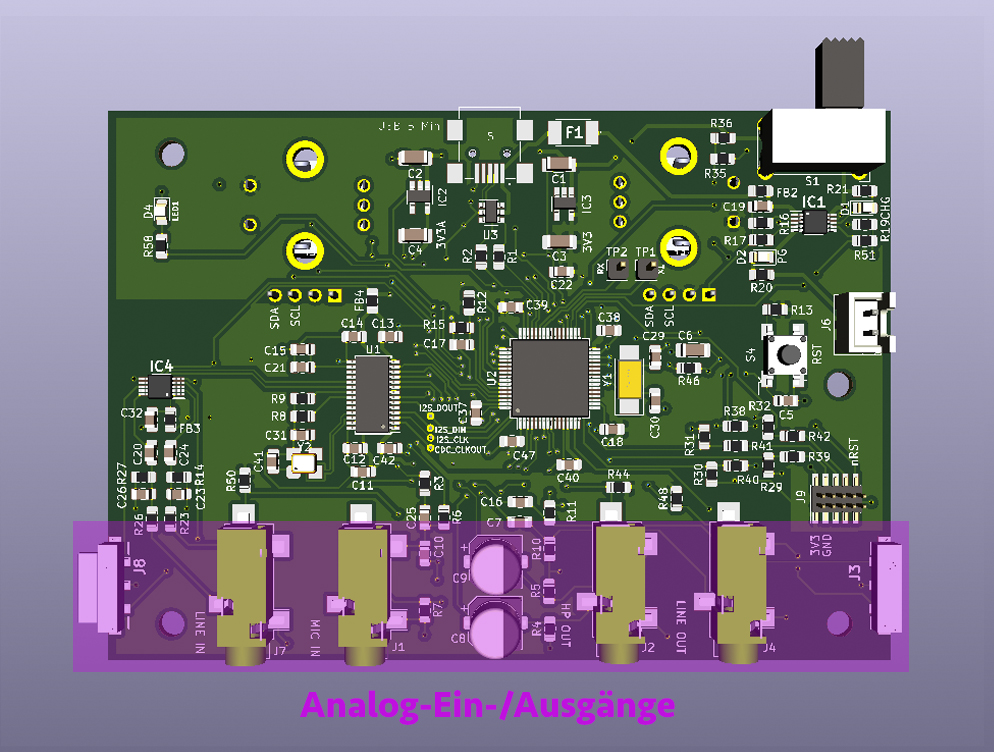
\includegraphics[scale=0.37]{../graphics/PCB-Layout_INOUT.jpg}
 \caption{Die Audio-Ein- und -Ausgänge mit 2x2 Mini-Jack Buchsen und 2 AVX-Verbinder für die Board-to-Board Verbindung}
\label{fig:PCB_INOUT}
\end{center}
\end{figure}

Mit dem Gedanken das Board später mit einem Gehäuse zu ergänzen sind die Ein-/Ausgänge, speziell die AVX-Stecker für die Board-zu-Board Verbindung, möglichst nahe am Rand platziert. Um es einheitlich zu halten, dient die untere Kante als Audio-Interface und die obere Kante als Digital-/Power-Interface. 

\begin{figure} [H]
\begin{center}
 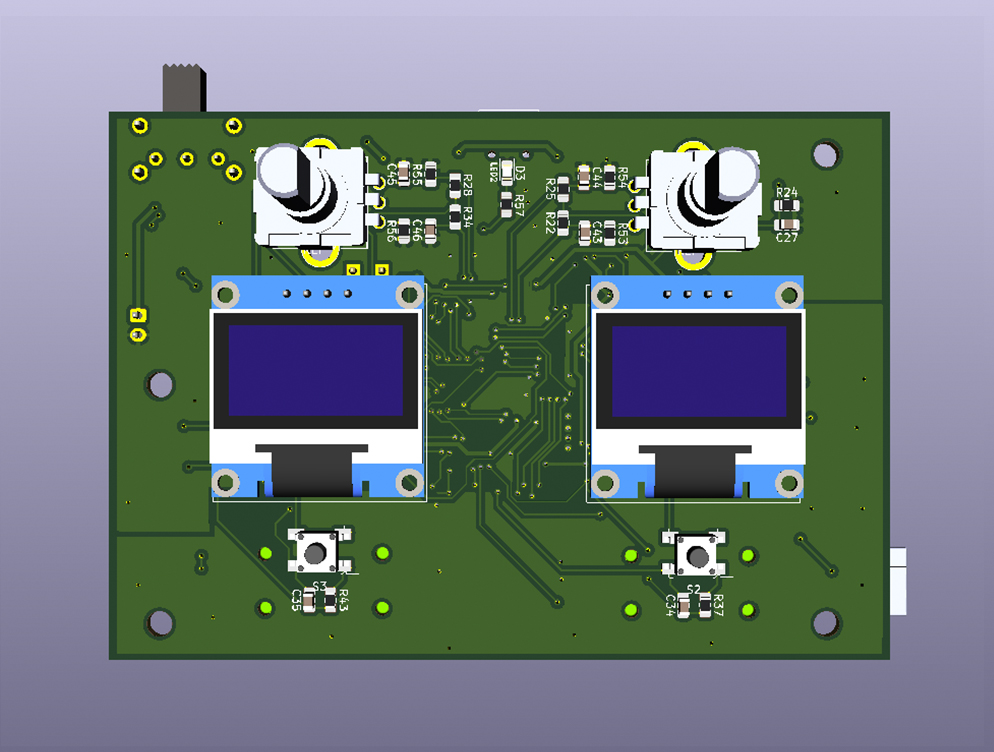
\includegraphics[scale=0.37]{../graphics/PCB-Layout_GUI.jpg}
 \caption{Die Bedienoberfläche mit je zwei Rotary-Encodern, Buttons und OLED-Displays}
\label{fig:PCB_GUI}
\end{center}
\end{figure}

Um Kosten zu sparen sind die Bedienelemente für das Benutzer-Interface gleich auf der Rückseite des PCBs angebracht.